\documentclass{ximera}

\newcommand{\RR}{\mathbb R}
\renewcommand{\d}{\,d}
\newcommand{\dd}[2][]{\frac{d #1}{d #2}}
\renewcommand{\l}{\ell}
\newcommand{\ddx}{\frac{d}{dx}}
\newcommand{\dfn}{\textbf}
\newcommand{\eval}[1]{\bigg[ #1 \bigg]}

\author{Jim Talamo}

\outcome{Define a series.}
\outcome{Recognize a geometric series.}
\outcome{Recognize a telescoping series.}
\outcome{Compute the sum of a geometric series.}
\outcome{Compute the sum of a telescoping series.}

\title[Dig-In:]{Series}

\begin{document}
\begin{abstract}
We discuss convergence results for geometric series and telescoping series.
\end{abstract}
\maketitle

Suppose that we have a \emph{series} $\sum_{k=k_0}^{\infty} a_k$ and have to determine whether it converges or diverges.  To answer this question, we define a new \emph{sequence} $\{s_n\}_{n=k_0}$ where $s_n = \sum_{k=k_0}^{n}$ for all $n \geq k_0$.  We saw previously that
 
 \begin{itemize}
\item the series $\sum_{k=k_0}^\infty a_k$ \dfn{converges} if and only if $\lim_{n\to\infty} s_n$ exists.  
\item the series $\sum_{k=k_0}^\infty a_k$ \dfn{diverges} if and only if $\lim_{n\to\infty} s_n$ does not exist.  
\end{itemize}

The most straightforward way to determine whether $\lim_{n \to \infty} s_n$ exists is to have an explicit formula for the $n$-th term $s_n$.  Note that this is not an easy task; for example, can you find a formula for $s_n$ for the series $\sum_{k=1}^{\infty} \frac{1}{k}$? It's not too hard to write out the first several terms in the sequence $\{s_n\}_{n=1}$, but try to find an explicit formula that describes the next term in the list.

\section{A recursive formula for $s_n$}
As it turns out, there is always a recursive formula for $s_n$.  For the sake of example, suppose that we want to consider $\sum_{k=1}^{\infty} a_k$.  Let's write out the formula for $s_n$.

\[
s_n = a_1+a_2+a_3+\ldots+a_{n-1}+a_n
\]


We can make an observation by considering $s_{n-1}$ in a similar way.

\[
s_{n-1} = a_1+a_2+a_3+\ldots+a_{n-1}
\]

Now returning to our expression for $s_n$, we can make an observation. 
\begin{image}
  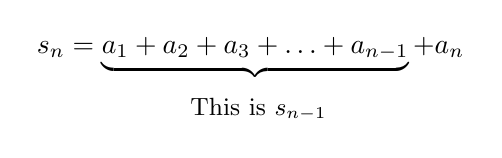
\begin{tikzpicture}
        \node at (0,0) {
          $s_n = \underbrace{a_1+a_2+a_3 + \ldots + a_{n-1}}+ a_n$};
        \node at (.1,-.65) {\small{This is $s_{n-1}$}};
      
      \end{tikzpicture}
  \end{image}

We thus have the formula 

\[
s_n = s_{n-1}+a_n.
\]

If we apply this to the series $\sum_{k=1}^{\infty} \frac{1}{k}$, where $a_n = \frac{1}{n}$, the result read $s_n = s_{n-1} + \frac{1}{n}$.  This does not help us analyze whether $\lim_{n \to \infty} s_n$ actually exists.  Sometimes, however, we can find an \emph{explicit} formula for $s_n$, and we study two special types of series for which this is possible.

\section{Geometric series}
Recall that a \emph{geometric sequence} is a sequence for which the ratio of successive terms is constant.  If $\{a_n\}_{n=n_0}$ is such a sequence, then there are constants $a \ne 0$ and $r$ for which $a_n = a\cdot r^n$.  

This generates the ordered list

\[
ar^{n_0} , ar^{n_0+1}, ar^{n_0+2}, \ldots
\]

<<<<<<< HEAD
and we have a result for the limits of these types of sequences, which we now recall.
=======
Note that the \emph{limit} of this new sequence is exactly the \emph{sum} of all of the terms in the old sequence!  Let's formalize the ideas in the last example with a definition.

\begin{definition}
Let $\{a_n\}_{n=n_0}$ be a sequence.  Let $s_n = \sum_{k=k_0}^n a_k$; the sequence $\{s_n\}_{n=k_0}$ is the called the
  \dfn{sequence of partial sums} of $\{a_n\}$.  

\begin{enumerate}
\item The series $\sum_{k=k_0}^\infty a_k$ \dfn{converges} if and only if $\lim_{n\to\infty} s_n$ exists.  Furthermore, if $\lim_{n\to\infty} s_n =L$, we say the series $\sum_{k=k_0}^\infty a_k$ converges to $L$. 
\item The series $\sum_{k=k_0}^\infty a_k$ \dfn{diverges} if and only if $\lim_{n\to\infty} s_n = \infty, \lim_{n\to\infty} s_n = -\infty$ or $\lim_{n\to\infty} s_n $ otherwise does not exist.  
\end{enumerate}
\end{definition}

The above definition really is assuring us that the symbols $\sum_{k=k_0} a_k$ and $\lim_{n \to \infty} s_n$ are exactly the same! However, this definition makes the content of the previous example more precise.  The major idea here is that we have techniques that we can use to determine whether limits exist and can even find what those limits are sometimes.  Since we are now able to recast the new question ``Can I sum all of the terms in a sequence?'' into the old question ``Does a sequence have a limit?", we can now utilize all of our previous techniques to analyze the sequence of partial sums.

\begin{remark}
Some texts take the $n$-th term in the sequence of partial sums to be found by summing the first $n$ terms in the original sequence.  With our convention, the lower index for both the original sequence and the sequence of partial sums will always be the same; that is, both sequences share a common domain.  In the case when the lower index is $k_0=1$, both conventions are equivalent.
\end{remark}

\begin{question}
  Using our new terminology, what can we say about the series $\sum_{k=1}^\infty \left(\frac{1}{2}\right)^k$ from the previous example?  \begin{prompt}The series     \wordChoice{\choice[correct]{converges}\choice{diverges}}, and
      $\sum_{n=1}^\infty \left(\frac{1}{2}\right)^n = \answer[given]{1}$.
  \end{prompt}
\end{question}
%\begin{definition}
%  A \dfn{series} is a sum of an infinite sequence.
%\end{definition}
%
%
%Let's start our investigation on this topic with a question (a little unfair, I know!).
%
%\begin{question}
%  Can the sum of an infinite number of terms be a finite value?
%  \begin{prompt}
%    \begin{multipleChoice}
%      \choice{no}
%      \choice[correct]{sometimes}
%    \end{multipleChoice}
%  \end{prompt}
%\end{question}
%As we will see, the answer is ``sometimes.''  Believe it or not, you
%have been working with infinite sums of numbers (also called
%\textit{series}) for a long time. Consider the number
%\[
%\frac{1}{3} = 0.3333333333\dots .
%\]
%This is the infinite sum of the geometric sequence
%$(a_n)_{n=1}^\infty$ where $a_n = \frac{3}{10^{n}}$, as
%\begin{align*}
%  \sum_{n=1}^\infty 3\cdot \frac{1}{10^{n}} &= 0.3 + 0.03+0.003+ 0.0003+ 0.00003+ \cdots\\
%  &= \frac{3}{10} + \frac{3}{10^2} + \frac{3}{10^3} + \frac{3}{10^4} + \frac{3}{10^5} + \cdots\\
%  &=\frac{1}{3}.
%\end{align*}

%%%%%%%%%%%%%%%%%%%%%%

%MOVE TO EXERCISES

%%%%%%%%%%%%%%%%%%%%%%

%We can sum other geometric series to finite values as well. Consider
%\[
%\sum_{n=1}^\infty \left(\frac{1}{4}\right)^n =
%\frac{1}{4} + \left(\frac{1}{4}\right)^2 + \left(\frac{1}{4}\right)^3 + \left(\frac{1}{4}\right)^4 + \cdots 
%\]
%A very clever method of summing this sequence is as follows. Consider
%an equilateral triangle with area $1$:
%\begin{image}[1in]
%  \begin{tikzpicture}[scale=3,rounded corners=.5pt]      
%    \tkzDefPoint(0,1){A1} 
%    \tkzDefPoint(-.58,0){A2}
%    \tkzDefPoint(.58,0){A3}
%    \draw[penColor,very thick] (A1)--(A2)--(A3)--cycle;
%  \end{tikzpicture}
%\end{image}
%We can break this triangle into $4$ congruent triangles, each of area
%$1/4$:
%\begin{image}[1in]
%  \begin{tikzpicture}[scale=3,rounded corners=.5pt]      
%    \tkzDefPoint(0,1){A1} 
%    \tkzDefPoint(-.58,0){A2}
%    \tkzDefPoint(.58,0){A3}
%    \draw[penColor,very thick] (A1)--(A2)--(A3)--cycle;
%
%    \tkzDefPoint(0,0){B1} 
%    \tkzDefPoint(-.29,.5){B2}
%    \tkzDefPoint(.29,.5){B3}
%    \draw[penColor,fill=fill1,very thick] (B1)--(B2)--(B3)--cycle;
%  \end{tikzpicture}
%\end{image}
%We can break the upper triangle into $4$ more congruent triangles, each
%with area $(1/4)^2$:
%\begin{image}[1in]
%  \begin{tikzpicture}[scale=3,rounded corners=.5pt]      
%    \tkzDefPoint(0,1){A1} 
%    \tkzDefPoint(-.58,0){A2}
%    \tkzDefPoint(.58,0){A3}
%    \draw[penColor,very thick] (A1)--(A2)--(A3)--cycle;
%
%    \tkzDefPoint(0,0){B1} 
%    \tkzDefPoint(-.29,.5){B2}
%    \tkzDefPoint(.29,.5){B3}
%    \draw[penColor,fill=fill1,very thick] (B1)--(B2)--(B3)--cycle;
%
%    \tkzDefPoint(0,.5){C1} 
%    \tkzDefPoint(-.14,.75){C2}
%    \tkzDefPoint(.14,.75){C3}
%    \draw[penColor,fill=fill1,very thick] (C1)--(C2)--(C3)--cycle;
%  \end{tikzpicture}
%\end{image}
%Repeating this process, we find:
%\begin{image}[1in]
%  \begin{tikzpicture}[scale=3,rounded corners=.5pt]      
%    \tkzDefPoint(0,1){A1} 
%    \tkzDefPoint(-.58,0){A2}
%    \tkzDefPoint(.58,0){A3}
%    \draw[penColor,very thick] (A1)--(A2)--(A3)--cycle;
%
%    \tkzDefPoint(0,0){B1} 
%    \tkzDefPoint(-.29,.5){B2}
%    \tkzDefPoint(.29,.5){B3}
%    \draw[penColor,fill=fill1,very thick] (B1)--(B2)--(B3)--cycle;
%
%    \tkzDefPoint(0,.5){C1} 
%    \tkzDefPoint(-.14,.75){C2}
%    \tkzDefPoint(.14,.75){C3}
%    \draw[penColor,fill=fill1,very thick] (C1)--(C2)--(C3)--cycle;
%
%    \tkzDefPoint(0,.75){D1} 
%    \tkzDefPoint(-.07,.875){D2}
%    \tkzDefPoint(.07,.875){D3}
%    \draw[penColor,fill=fill1,very thick] (D1)--(D2)--(D3)--cycle;
%
%    \tkzDefPoint(0,.875){E1} 
%    \tkzDefPoint(-.04,.94){E2}
%    \tkzDefPoint(.04,.94){E3}
%    \draw[penColor,fill=fill1,very thick] (E1)--(E2)--(E3)--cycle;
%
%    \tkzDefPoint(0,.94 ){F1} 
%    \tkzDefPoint(-.02,.97){F2}
%    \tkzDefPoint(.02,.97){F3}
%    \draw[penColor,fill=fill1,very thick] (F1)--(F2)--(F3)--cycle;
%  \end{tikzpicture}
%\end{image}
%where the area of the shaded triangles is our geometric series:
%\[
%\frac{1}{4} + \left(\frac{1}{4}\right)^2 + \left(\frac{1}{4}\right)^3 + \left(\frac{1}{4}\right)^4 + \cdots 
%\]
%The area is clearly finite (it is between $0$ and $1$!). What is the
%shaded area? Well, if you look at any ``row'' of the triangle, we've
%shaded in exactly one third of the row. Hence we've shaded in one third of
%the entire area, so we see
%\[
%\frac{1}{3}=\frac{1}{4} + \left(\frac{1}{4}\right)^2 + \left(\frac{1}{4}\right)^3 + \left(\frac{1}{4}\right)^4 + \cdots 
%\]
%While this is a very cool argument, it doesn't generalize well. Let's consider
% an argument that will apply to more settings.
%
%\begin{example}
%  Explain why
%  \[
%  \frac{1}{3}=\frac{1}{4} + \left(\frac{1}{4}\right)^2 + \left(\frac{1}{4}\right)^3 + \left(\frac{1}{4}\right)^4 + \cdots 
%  \]
%  \begin{explanation}
%    Here is the idea: first, ``name'' your sum $S$.
%    \[
%    S = \frac{1}{4} + \left(\frac{1}{4}\right)^2 + \left(\frac{1}{4}\right)^3 + \left(\frac{1}{4}\right)^4 + \cdots 
%    \]
%    Now, multiply $S$ by $\frac{1}{4}$ and write this suggestively under $S$.
%    \begin{align*}
%      S &= \frac{1}{4} + \left(\frac{1}{4}\right)^2 + \left(\frac{1}{4}\right)^3 + \left(\frac{1}{4}\right)^4 + \cdots\\
%     \left(\frac{1}{4}\right)S &=   \left(\frac{1}{4}\right)^2 + \left(\frac{1}{4}\right)^3 + \left(\frac{1}{4}\right)^4 + \left(\frac{1}{4}\right)^5+ \cdots
%    \end{align*}
%    subtracting the lower line from the upper line we find
%    \begin{align*}
%      S - \left(\frac{1}{4}\right)S &=  \frac{1}{4}\\
%      S(1-\frac{1}{4}) &= \frac{1}{4}\\
%      S &= \frac{\frac{1}{4}}{1-\frac{1}{4}}\\
%      S &= \frac{1}{3}.
%    \end{align*}
%  \end{explanation}
%\end{example}
%
%This is a good method for understanding infinite sums of geometric
%sequences (assuming you know the sequence sums to a finite value).
%
%To make this precise, we need some definitions. 

\section{Two special types of series}
The definitions above give us a way to determine whether a given series converges.  In fact, to determine whether $\sum_{k=k_0} a_k$ converges, we can do the following.

\begin{itemize}
\item[1.] Consider the associated sequence $\{s_n\}$ of partial sums.
\item[2.] Try to find an explicit formula for the term $s_n$.  If you can find such a formula, analyze $\lim_{n \to \infty s_n}$.  
\begin{itemize}
\item If the limit exists, $\sum_{k=k_0}^{\infty} a_k$ converges, and if we can determine that $\lim_{n \to \infty} s_n =L$, then $\sum_{k=k_0} a_k=L$.  \item If  $\lim_{n \to \infty} s_n$ does not exist, then $\sum_{k=k_0} a_k$ diverges.
\end{itemize}
\item[3.] If an explicit formula for $s_n$ cannot be found, further analysis is needed.  We'll expound on this in later sections.
\end{itemize}
>>>>>>> c4bcc6d632e2210509df494251f9d576bbe3e863

\begin{theorem}
  Given a geometric sequence $\{a_n\}_{n=n_0}$ where $a_n = a \cdot r^{n}$,
  \[
  \lim_{n\to\infty} a_n =
  \begin{cases}
    0 &\text{if $|r|<1$,}\\
    1 &\text{if $r=1$,}\\
    \text{DNE} &\text{if $|r|>1$ or $r=-1$.}
  \end{cases}
  \]
\end{theorem}

We can now think of adding together the terms of a geometric sequence.

\begin{definition}
  A \dfn{geometric series} is a series of the form $\sum_{k=k_0}^\infty ar^k$
  for some real numbers $a \ne 0$ and $r$.
\end{definition}

Before exploring when such a series converges, note that sometimes, some preliminary algebra is necessary to recognize a series as geometric.

\begin{example}
The series $\sum_{k=4}^\infty \frac{2^{2k+1}}{3^k}$ \wordChoice{\choice[correct]{is}\choice{is not}} geometric since $a_k =\frac{2^{2k+1}}{3^k}$ \wordChoice{\choice[correct]{can}\choice{cannot}} be brought into the form $a \cdot r^k$.  

Using the laws of exponents shows us:

\[
\frac{2^{2k+1}}{3^k} = \frac{2^{2k} \cdot 2^1}{3^k}= 2 \cdot \frac{\left(2^{k}\right)^2}{3^k} = 2 \cdot \frac{4^k}{3^k} = 2 \cdot \left(\frac{4}{3}\right)^k.
\]
Indeed, $a= \answer[given]{2}$ and $r = \answer[given]{\frac{4}{3}}$.
\end{example}

\begin{example}
The series $\sum_{k=0}^\infty k^2 \left(\frac{1}{2}\right)^k$ \wordChoice{\choice{is}\choice[correct]{is not}} geometric since $a_k = \answer[given]{k^2 \cdot \frac{1}{2}^k}$ \wordChoice{\choice{can}\choice[correct]{cannot}} be brought into the form $a \cdot r^k$.  Indeed, the coefficient, $k^2$, is not the same for each term in the series.
\end{example}

We can now try to determine when adding together the terms in such a series is possible; that is, we can explore for which values of $a$ and $r$ the \emph{series} $\sum_{k=n_0}^{\infty} a_k$ converges.  

\begin{model}
 Let $r \neq 1$ and consider the geometric series $\sum_{k=0}^\infty a r^k$, and let $s_n = \sum_{k=0}^{\infty} a r^k $.  We find an explicit formula for the term $s_n$.
  
  \begin{explanation}
First, note that the sum above represents the attempt to add all of the terms in the sequence $\{a_n\}_{n=0}$, where $a_n =  r^n$.  Let's start by writing out the first several terms in the sequence $\{a_n\}$.  

\[
a_0 = 1 , \qquad a_1 = r, \qquad a_2 = r^2 , \qquad \ldots ,
\]
    \begin{align*}
      s_0 &= a_0 = 1 \\
      s_1 &= 1 + 1r\\
      s_2 &= 1 + r + r^2\\
      &\vdots\\
      s_n &= 1 + r + r^2 + \dots + r^n
    \end{align*}
The general difficulty for finding a closed formula for $s_n$ arises because, without specifying what $n$ is, we cannot actually perform the indicated addition.  However, there's a nice trick we can exploit here.

We start by multiplying $s_n$ by the common ratio $r$.
    \begin{align*}
      s_n   &= 1 + r + r^2 + \dots + r^n\\
      r s_n &= ~ \phantom{ 1 + } r + r^2 + \dots + r^n + r^{n+1}
    \end{align*}
Now, we can subtract away the middle terms.

 \[     \begin{array}{rl}
      s_n   &= 1 + \cancel{ r + r^2 + \dots + r^n}\\
 -\left(  \phantom{ r^{n+1}} r s_n \right.&=~ \left. \phantom{  1 +  } \cancel{r + r^2 + \dots + r^n} + r^{n+1}\right) \\
 \hline 
     s_n - r s_n &= 1 \phantom{  +  r + r^2 + \dots + r^n } ~ - r^{n+1}\\
    \end{array}
 \]   
 
 We can now solve for $s_n$.
 
     \begin{align*}
      s_n - r s_n &= 1 - r^{n+1}\\
      s_n(1-r)    &= 1 - r^{n+1}\\
      s_n &= \frac{1 - r^{n+1}}{1-r}.
    \end{align*}
    Since $s_n$ is \textbf{always} a finite sum, and $r \ne 1$, there is no issue
    with manipulating it the way we did.
  \end{explanation}
\end{model}

From our work above, we see that the $n$-th partial sum of the
geometric series $a_n = r^n$ is
\[
s_n = \sum_{k=0}^{n} r^k= \frac{1 - r^{n+1}}{1-r}.
\]
We now have an \emph{explicit} formula so we can determine for which values of $r$ the limit $\lim_{n \to \infty} s_n$ exists.  First, note that the limit in question, $\lim_{n \to \infty} r^{n+1}$ is the limit of a \emph{geometric} sequence.  In fact, 

\begin{itemize}
\item if $-1<r<1$, then $\lim_{n \to \infty} r^{n+1}$ \wordChoice{\choice[correct]{exists}\choice{does not exist}}.
\item if $r>1$ or $r\le -1$, then $\lim_{n \to \infty} r^{n+1}$ \wordChoice{\choice{exists}\choice[correct]{does not exist}}.
\end{itemize}

In fact, if $r>1$, the $r^{n+1}$ is not bounded above.  If $r=-1$, the $r^{n+1}$ is bounded, but the terms oscillate between $-1$ and $1$.  If $r>1$, the terms $r^{n+1}$ both oscillate in sign and become arbitrarily large in magnitude.

The above formula covers every case except when $r= 1$, but notice that  $$\sum_{k=0}^n 1 = n+1,$$ so if $r=1$, $s_n = \answer[given]{n+1}$ and $\lim_{n \to \infty} s_n = \infty$, so $\sum_{k=0}^{\infty} 1$ diverges. 

When $-1<r<1$, note $\lim_{n \to \infty} r^{n+1}=0$, so in this case,     \[
    \lim_{n\to\infty}\frac{1 - r^{n+1}}{1-r} = \frac{1-\answer[given]{0}}{1-r}.
    \]

By noting that $\sum_{k=0}^n ar^k = a \sum_{k=0}^n r^k$, we can combine this observation with the above argument and write the result in a theorem.

\begin{theorem}
  The geometric series $\sum_{k= 0}^\infty a \cdot r^k$ 
  
  \begin{itemize} 
  \item converges to $\frac{a}{1-r}$ when $|r| < 1$.
  \item diverges if $|r| \geq 1$.  
  \end{itemize}
  \end{theorem}

There is a useful trick that allows us to find the sum of a convergent geometric series when the lower index does not start at $0$.  

\begin{example}
The series $\sum_{k=3}^{\infty} \left(\frac{2}{3}\right)^k$ is a geometric series with $r=\frac{2}{3}<1$, so it converges.  To find the value to which it converges, notice the following.

\begin{align*}
\sum_{k=3}^{\infty} \left(\frac{2}{3}\right)^k &=  \left(\frac{2}{3}\right)^3+ \left(\frac{2}{3}\right)^4+ \left(\frac{2}{3}\right)^5+\ldots \\
&= \left(\frac{2}{3}\right)^3 \cdot \left(1+ \frac{2}{3}+ \left(\frac{2}{3}\right)^2+\ldots\right) \\
&= \frac{8}{27}  \cdot  \sum_{k=0}^{\infty}\left(\frac{2}{3}\right)^k \\
&= \sum_{k=0}^{\infty} \frac{8}{27}  \cdot \left(\frac{2}{3}\right)^k
\end{align*}
This is now a geometric series whose lower index is $0$, so we can use the formula to find its value. Noting that $a=\answer[given]{ \frac{8}{27} }$ and $r= \frac{2}{3}$ gives:

\[
\sum_{k=3}^{\infty} \left(\frac{2}{3}\right)^k = \frac{8/27}{1-2/3} = \frac{8}{9}.
\]
\end{example}

We can easily generalize this example and doing so allows us to write down a more comprehensive theorem about geometric series.

\begin{theorem}
\index{series!geometric}\index{geometric series}\index{geometric series!convergence}\index{geometric series!divergence}
  The geometric series $\sum_{k= k_0}^\infty a \cdot r^k$ 
  
  \begin{itemize} 
  \item converges to $\frac{ar^{k_0}}{1-r}$ when $|r| < 1$.
  \item diverges if $|r| \geq 1$.  
  \end{itemize}
  \end{theorem}
 
\begin{example}
Let's take another look at the series that started off the section, $\sum_{k=1}^{\infty} \left(\frac{1}{2}\right)^k$.  Here, $a=\answer[given]{0}$, $r=\answer[given]{1/2}$ and $k_0 = \answer[given]{1}$.  Since $|r|<a$, the series \wordChoice{\choice[correct]{converges}\choice{diverges}}, and using the formula above, we have that

\[ \sum_{k=1}^{\infty} \left(\frac{1}{2}\right)^k = \frac{ar^{k_0}}{1-r} = \frac{1\cdot \frac{1}{2}}{1-1/2} =1.\]

This matches the earlier result!  
\end{example}

\begin{remark} 
Although we have mentioned it before, we mention it again here:

\begin{quote}
The lower index in a series does not affect whether the series converges or diverges, but if the series converges, it can affect the value to which the series converges.
\end{quote}
The formula listed above very explicitly shows exactly how the lower index $k_0$ affects the value to which a convergent geometric series converges.

\end{remark}

Now, try some questions to check your understanding of the above material.

\begin{question}
  Which of the following series converge?
  \begin{selectAll}
    \choice{$\sum_{k=0}^\infty \left(\frac{3}{2}\right)^k$}
    \choice[correct]{$\sum_{k=0}^\infty \left(\frac{-2}{3}\right)^k$}
    \choice[correct]{$\sum_{k=9}^\infty \left(\frac{1}{7}\right)^k$}
    \choice{$\sum_{k=1}^\infty (-1)^k$}
    \choice[correct]{$\sum_{k=-9}^\infty \left(\frac{1}{2}\right)^k$}    
  \end{selectAll}
  \begin{hint}
    The initial index doesn't matter as far as convergence is
    concerned, it is the ``tail'' of the sequence that determines
    convergence.
  \end{hint}
\end{question}

\begin{question}
Determine if the series $\sum_{k=2}^{\infty} 2^{3-2k}$ converges or diverges.  If it converges, give the value to which it converges.

\begin{explanation}
First, note that the series \wordChoice{\choice[correct]{is}\choice{is not}} geometric since the laws of exponents allow us to write the following.

\[
2^{3-2k} = \frac{2^3}{2^{2k}} = \frac{8}{\left(2^2\right)^k} =  8 \cdot \frac{1}{4^k} =  8 \cdot \frac{1^k}{4^k} =  8 \cdot \left(\frac{1}{4}\right)^k
\]

The series is geometric with $r = \answer[given]{1/4}$, and using the result $\sum_{k=k_0} ar^k = \frac{ar^{k_0}}{1-r}$ gives:

\[
\sum_{k=2}^{\infty} 2^{3-2k} =  8 \cdot \left(\frac{1}{4}\right)^k =  \frac{8 \cdot (1/4)^2}{1-1/4}  =  \answer[given]{\frac{2}{3}}.
\]
\end{explanation}

\end{question}    

\section{Telescoping series}
\index{series!telescoping}\index{telescoping series}

A second type of series for which we can find an explicit formula for $s_n$ are ``telescoping series''.  Rather than try to give a formal definition, we think of telescoping series are infinite sums for which the required addition required to find a formula for $s_n$ can be done so many of the intermediate terms naturally cancel.  An example will make this point more clear.

\begin{example}
  Evaluate the sum
  \[
  \sum_{k=1}^\infty\left(\frac{1}{k}-\frac{1}{k+1}\right).
  \]
  \begin{explanation}
It will help to write down the first few partial sums for this series.
\begin{image}
\begin{tikzpicture}
    \node at (0,0) {
      $\begin{aligned}
        s_1 &=	\frac11-\frac12 & & = 1-\frac12\\
        s_2 &=	\left(\frac11-\frac12\right) + \left(\frac12-\frac13\right) & & = 1-\frac13\\
        s_3 &=	\left(\frac11-\frac12\right) + \left(\frac12-\frac13\right)+\left(\frac13-\frac14\right) & &= 1-\frac14\\
        s_4 &=	\left(\frac11-\frac12\right) + \left(\frac12-\frac13\right)+\left(\frac13-\frac14\right) +\left(\frac14-\frac15\right)& &= 1-\frac15
      \end{aligned}$};
\end{tikzpicture}
\end{image}
For $s_2$ and beyond, note how most of the intermediate terms in each partial sum cancel out! In
general, we can notice from pattern recognition (specifically by looking at the denominator in each expression and comparing it to the index) that $s_n =$ \wordChoice{\choice{$1-\frac{1}{n}$},\choice[correct]{$1-\frac{1}{n+1}$}}. The sequence $\{s_n\}_{n=1}$ thus \wordChoice{\choice[correct]{converges}\choice{diverges}} since $\lim_{n \to \infty} s_n$ \wordChoice{\choice[correct]{exists}\choice{does not exist}}. Furthermore, since $\lim_{n\to\infty}s_n = \lim_{n\to\infty}\left(1-\frac1{n+1}\right) = \answer[given]1$, we conclude
that $\sum_{n=1}^\infty \left(\frac1n-\frac1{n+1}\right) = 1$.
  \end{explanation}
\end{example}

\begin{remark}
Finding the above formula required us to use pattern recognition.  Validating that the pattern must hold for \emph{all} terms in the sequence can be done formally by using an idea called \emph{mathematical induction}.  We leave it to the curious reader to explore this idea further if desired.
\end{remark}

We've just seen an example of a \dfn{telescoping series}. Informally,
a telescoping series is one in which the partial sums reduce to just a
finite sum of terms. In the last example, the partial sum $s_n$ only was the sum of two nonzero terms: 
\[
s_n = 1 - \frac{1}{n-1}.
\]

%\begin{example}
%Determine if the series $\sum_{n=1}^\infty \frac{2}{n^2+2n}$ converges or diverges.  If it converges, find the value to which it converges.
%
%\begin{explanation}
%All of the terms in the above sum are positive, so there is no convenient cancellation that will occur if we try to find a formula for $s_n$ yet.  However, we can use partial fractions to write
%  \[
%  \frac{2}{n^2+2n} = \frac{1}{n}-\frac{1}{n+2}.
%  \]  
%  Expressing the terms of $\{s_n\}$ now produces a pattern.  
%  \begin{image}
%    \begin{tikzpicture}
%      \node at (0,0) {
%        $\begin{aligned}
%          s_1 &= 1-\frac13 &&= 1-\frac13\\
%          s_2 &= \left(1-\frac13\right) + \left(\frac12-\frac14\right) &&= 1+\frac12-\frac13-\frac14\\
%          s_3 &= \left(1-\frac13\right) + \left(\frac12-\frac14\right)+\left(\frac13-\frac15\right) &&= 1+\frac12-\frac14-\frac15\\
%          s_4 &= \left(1-\frac13\right) + \left(\frac12-\frac14\right)+\left(\frac13-\frac15\right)+\left(\frac14-\frac16\right) &&= 1+\frac12-\frac15-\frac16\\
%          s_5 &= \left(1-\frac13\right) + \left(\frac12-\frac14\right)+\left(\frac13-\frac15\right)+\left(\frac14-\frac16\right)+\left(\frac15-\frac17\right) &&= 1+\frac12-\frac16-\frac17\\
%        \end{aligned}$};
%    \end{tikzpicture}
%  \end{image}
%\textbf{I WANT TO WRITE SOMETHING ABOUT THE DENOMINATORS BEING 2 APART, WHICH IS WHYIT TAKES WRITING OUT 3 TERMS UNTIL TO EXHIBIT THE EVENTUAL PATTERN.  CAN ANYONE HELP ME WORD THIS?}
%
%We again have a telescoping series. In each partial sum, most of the intermediate 
%  terms cancel and we obtain the formula
%  \[
%  s_n =1+\frac12-\frac1{n+1}-\frac1{n+2}.
%  \]
%  Taking limits allows us to determine the convergence of the series. Since
%  \[
%  \lim_{n\to\infty}s_n = \lim_{n\to\infty} \left(1+\frac12-\frac1{n+1}-\frac1{n+2}\right) = \frac32,
%  \]
%we conclude that
%  \[
%  \sum_{n=1}^\infty \frac1{n^2+2n} = \frac32.
%  \]
%\end{explanation}
%\end{example}



\begin{example}
Determine if the series $\sum_{k=1}^\infty \ln\left(\frac{k+1}{k}\right)$ converges or diverges. 
 
\begin{explanation}
We begin by writing the first few partial sums of the series:
\begin{align*}
s_1 &= \ln\left(2\right) \\
s_2 &= \ln\left(2\right)+\ln\left(\frac32\right) \\
s_3 &= \ln\left(2\right)+\ln\left(\frac32\right)+\ln\left(\frac43\right) \\
s_4 &= \ln\left(2\right)+\ln\left(\frac32\right)+\ln\left(\frac43\right)+\ln\left(\frac54\right) 
\end{align*}
At first, it doesn't look like we will have much luck writing this as a telescoping series, but noting that $ \ln\left(\frac{n+1}{n}\right) = \ln(n+1)-\ln(n)$ allows us to write out terms of $s_n$ in a more convenient way.

  \begin{image}
    \begin{tikzpicture}
      \node at (0,0) {
        $\begin{aligned}
          s_1 &= \ln(2)-\ln(1) &&= \ln(2)\\
          s_2 &= \left( \ln(3)-\ln(2)\right) + \left( \ln(2)-\ln(1)\right) &&= \ln(3)\\
          s_3 &= \left( \ln(4)-\ln(3)\right) + \left( \ln(3)-\ln(2)\right) + \left( \ln(2)-\ln(1)\right) &&= \ln(4)\\
%          s_4 &=  \left( \ln(5)-\ln(4)\right) +\left( \ln(4)-\ln(3)\right) + \left( \ln(3)-\ln(2)\right) + \left( \ln(2)-\ln(1)\right) &&= \ln(5)\\
        \end{aligned}$};
    \end{tikzpicture}
  \end{image}
  
  

%At first, this does not seem helpful, but recall the logarithmic rule
%$\ln(x)+\ln(y) = \ln (x\cdot y)$. Applying this rule to $S_4$ gives:
%\begin{align*}
%S_4 &= \ln\left(2\right)+\ln\left(\frac32\right)+\ln\left(\frac43\right)+\ln\left(\frac54\right) \\
%&= \ln\left(\frac21\cdot\frac32\cdot\frac43\cdot\frac54\right)\\
%&= \ln\left(5\right).

We can conclude that $s_n =\answer[given]{\ln (n+1)}$ and analyze $\lim_{n \to \infty} s_n$.  

Since $\lim_{n\to\infty}s_n=\answer[given]{\infty}$, $\sum_{k=1}^\infty \ln\left(\frac{k+1}{k}\right)$ diverges.
\end{explanation}
\end{example}


%%%%%%%%%%%%%%%%%%%%%%%%%%%%%%
\section{Summary}
Now that we have seen two special types of series for which we can find an explicit formula for the $n$-th term in the sequence of partial sums, it helps to summarize the logic that we employed.

\begin{itemize}
\item[1.] Consider the associated sequence $\{s_n\}$ of partial sums.
\item[2.] Try to find an explicit formula for the term $s_n$.  If you can find such a formula, analyze $\lim_{n \to \infty s_n}$.  
\begin{itemize}
\item If the limit exists, $\sum_{k=k_0}^{\infty} a_k$ converges, and if we can determine that $\lim_{n \to \infty} s_n =L$, then $\sum_{k=k_0} a_k=L$.  \item If  $\lim_{n \to \infty} s_n$ does not exist, then $\sum_{k=k_0} a_k$ diverges.
\end{itemize}
\end{itemize}


\end{document}
